\section{Questões}
\label{sec:questoes}

Esse capítulo é composto por respostas diretas às perguntas na descrição do trabalho. A explicação mais detalhada do funcionamento e as decisões de arquitetura da simulação são expostas na sessão \ref{sec:simulacao}.

\subsection{Discretização das Equações de Movimento}

\begin{questao}
Discretize as equações de movimento (Eqs. \ref{eq:quest-1.6} e \ref{eq:quest-1.7}) utilizando o método de Euler com passo $\Delta t$.
Apresente explicitamente as expressões para $x_{n+1}$ e $v_{n+1}$ em termos de $x_n$, $v_n$ e demais parâmetros do modelo.

\begin{equation}
    \label{eq:quest-1.6}
    m\frac{dv}{dt} = \begin{cases}
        -mg - \beta_\uparrow(x)v - \lambda_\uparrow(x)v^2, & v > 0\\
        -mg - \beta_\downarrow(x)v + \lambda_\downarrow(x)v^2, & v < 0\\
    \end{cases}
\end{equation}

\begin{equation}
    \label{eq:quest-1.7}
    \frac{dx}{dt} = v
\end{equation}
\end{questao}

Aplicando o método de Euler explícito, cada derivada é aproximada por uma diferença finita de primeira ordem:
\begin{equation*}
    \frac{df}{dt}\bigg|_{t_n} \approx \frac{f_{n+1} - f_n}{\Delta t}
\end{equation*}

Da Eq.~\ref{eq:quest-1.7}, obtém-se diretamente a atualização da posição:
\begin{equation}
    \label{eq:euler-x}
    x_{n+1} = x_n + v_n\,\Delta t
\end{equation}

Da Eq.~\ref{eq:quest-1.6}, isolando $v_{n+1}$:
\begin{equation}
    \label{eq:euler-v}
    v_{n+1} = \begin{cases}
        \displaystyle v_n - g\,\Delta t
            - \frac{\Delta t}{m}\Bigl[\beta_\uparrow(x_n)\,v_n + \lambda_\uparrow(x_n)\,v_n^2\Bigr],
        & v_n > 0 \\[10pt]
        \displaystyle v_n - g\,\Delta t
            - \frac{\Delta t}{m}\Bigl[\beta_\downarrow(x_n)\,v_n - \lambda_\downarrow(x_n)\,v_n^2\Bigr],
        & v_n < 0
    \end{cases}
\end{equation}

onde os coeficientes são avaliados na posição $x_n$ do instante anterior:
\begin{align}
    \beta_\uparrow(x_n)   &= \beta_0\,e^{-x_n/H},             &
    \lambda_\uparrow(x_n) &= \lambda_0\,e^{-x_n/H},           \label{eq:coef-up}\\
    \beta_\downarrow(x_n)  &= r_\beta\,\beta_\uparrow(x_n),    &
    \lambda_\downarrow(x_n)&= r_\lambda\,\lambda_\uparrow(x_n) \label{eq:coef-down}
\end{align}

A condição de parada da integração é $x_{n+1} < 0$, que indica que a partícula atingiu o solo.

\subsection{Análise dos Parâmetros na Subida}

\begin{questao}
Faça uma análise gráfica do comportamento dos parâmetros $\beta_\uparrow$ e $\gamma_\uparrow$ em função de $x$, para diferentes
valores dos parâmetros $\beta_0$, $\gamma_0$ e $H$. Discuta como as variações nesses parâmetros influenciam as curvas obtidas.
\end{questao}

Ambos os coeficientes compartilham a mesma dependência espacial,
\begin{equation}
    \beta_\uparrow(x) = \beta_0\,e^{-x/H}, \qquad \gamma_\uparrow(x) = \gamma_0\,e^{-x/H},
\end{equation}
de modo que a análise de $\beta_\uparrow$ é inteiramente análoga à de $\gamma_\uparrow$, com $\gamma_0$ no lugar de $\beta_0$. A Fig.~\ref{fig:beta-up-variation} apresenta as curvas $\beta_\uparrow(x)$ em dois cenários.

\textbf{Variação de $\beta_0$ (painel esquerdo).}  Com $H = 2{,}0\,\text{m}$ fixo, as curvas diferem apenas em amplitude: multiplicar $\beta_0$ por um fator $k$ escala o coeficiente por $k$ em \emph{toda} a faixa de alturas, sem alterar a taxa de decaimento. Fisicamente, $\beta_0$ representa a intensidade do arrasto ao nível do solo ($x = 0$); aumentá-lo eleva o arrasto proporcionalmente em todas as alturas.

\textbf{Variação de $H$ (painel direito).} Com $\beta_0 = 1{,}25\,\text{kg/s}$ fixo, o parâmetro $H$ controla a \emph{altura de escala} do decaimento. Para valores pequenos de $H$ (e.g.\@ $H = 1{,}0\,\text{m}$), o coeficiente cai rapidamente com a altitude - o arrasto é intenso próximo ao solo, mas torna-se desprezível já a poucos metros. Para valores grandes de $H$ (e.g.\@ $H = 6{,}0\,\text{m}$), o decaimento é lento e o arrasto permanece relevante ao longo de uma faixa maior de alturas. Esse comportamento é análogo ao de uma atmosfera exponencial, em que $H$ representa a escala de altura da densidade do ar.

\begin{figure}[!htb]
    \centering
    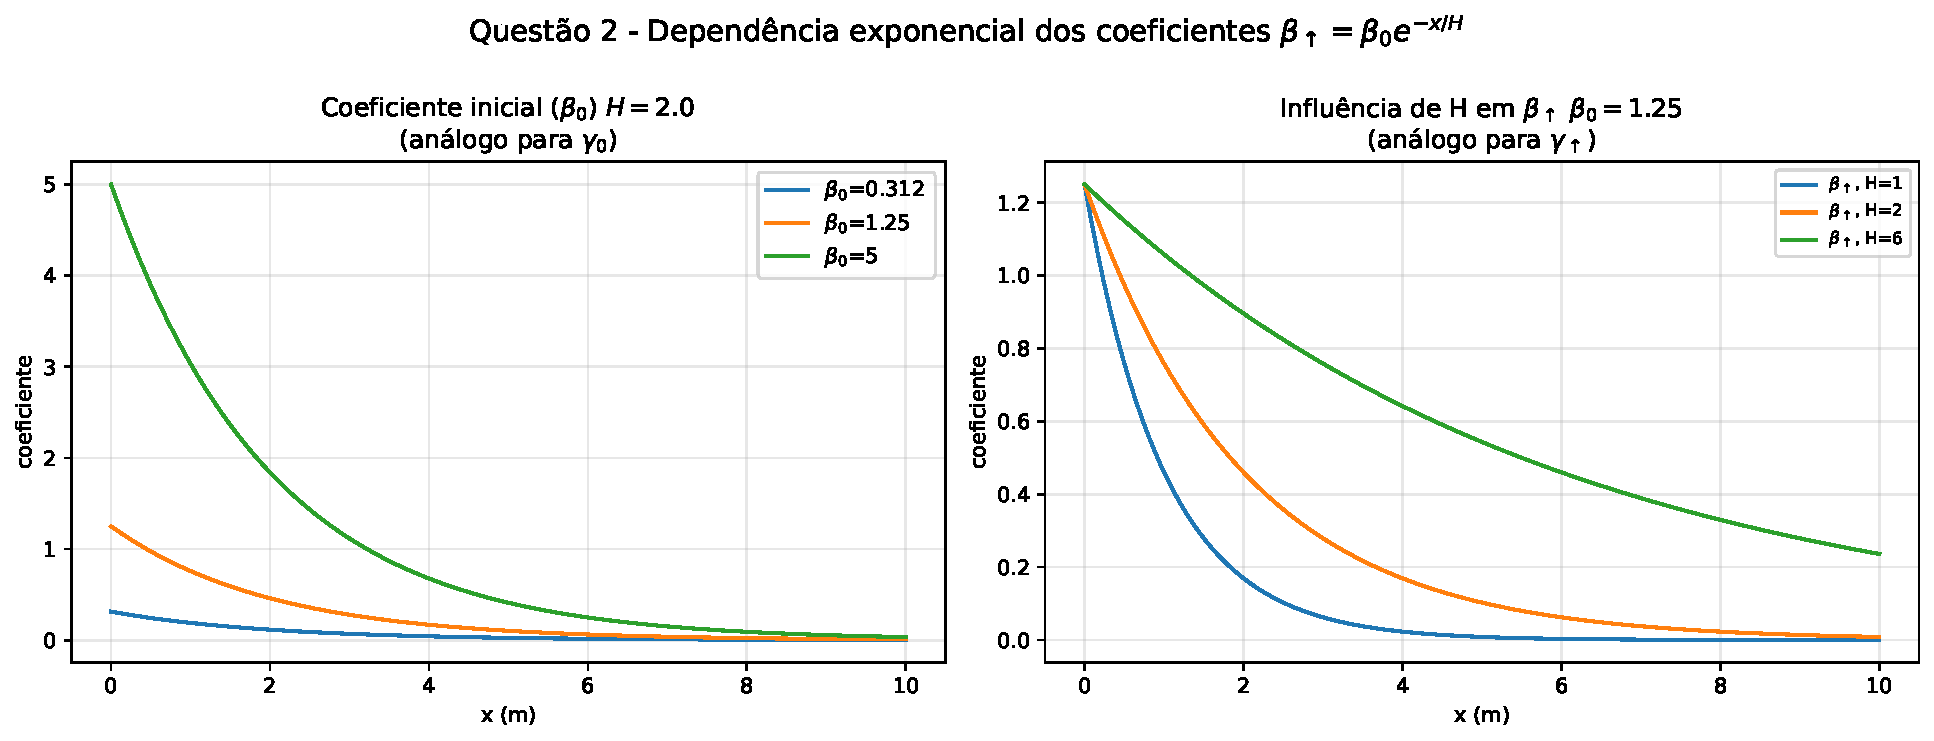
\includegraphics[width=\linewidth]{Imagens/questao2_beta_up_variation.pdf}
    \caption{Variação do $\beta_\uparrow$ pela altura}
    \label{fig:beta-up-variation}
\end{figure}


\subsection{Análise dos Parâmetros na Descida}

\begin{questao}
Faça uma análise gráfica do comportamento dos parâmetros $\beta_\downarrow$ e $\gamma_\downarrow$ em função de $x$, considerando
diferentes cenários para os parâmetros, tais como $r_\beta > 0$, $r_\beta < 0$, $r_\gamma > 0$ e $r_\gamma < 0$. Discuta como
essas diferentes condições influenciam as curvas obtidas.
\end{questao}

Os coeficientes de descida são definidos como múltiplos dos de subida:
\begin{equation}
    \beta_\downarrow(x) = r_\beta\,\beta_\uparrow(x) = r_\beta\,\beta_0\,e^{-x/H}, \qquad
    \gamma_\downarrow(x) = r_\gamma\,\gamma_0\,e^{-x/H},
\end{equation}
portanto o perfil espacial de decaimento exponencial é idêntico ao da subida; o que muda é o \emph{sinal e módulo} de $r_\beta$ (e analogamente $r_\gamma$). A Fig.~\ref{fig:beta-down-variation} ilustra $\beta_\downarrow(x)$ para $r_\beta \in \{-2,\,-1,\,0,\,+1,\,+2\}$ com $\beta_0 = 1{,}25\,\text{kg/s}$ e $H = 2{,}0\,\text{m}$.

\textbf{$r_\beta > 0$ (curvas sólidas acima do zero).} $\beta_\downarrow$ é positivo, tal como $\beta_\uparrow$. Como na descida $v < 0$, a força linear de arrasto $-\beta_\downarrow v$ aponta para cima (sentido oposto à velocidade), desacelerando a partícula. Quanto maior $r_\beta$, maior a intensidade dessa frenagem e menor a velocidade de impacto.

\textbf{$r_\beta = 0$.} O coeficiente linear de descida é nulo em toda a faixa de alturas: apenas o arrasto quadrático e a gravidade atuam durante a descida.

\textbf{$r_\beta < 0$ (curvas tracejadas abaixo do zero).} $\beta_\downarrow$ torna-se negativo. Nesse caso, a força $-\beta_\downarrow v = |\beta_\downarrow|\,|v|$ aponta para \emph{baixo} (mesma direção da velocidade), acelerando a partícula durante a descida. Fisicamente, esse cenário poderia representar, por exemplo, um efeito de sustentação ou um fluido ativo; do ponto de vista do modelo, ele reduz o tempo de descida e aumenta a velocidade de impacto em relação ao caso sem arrasto.

Em todos os cenários, o perfil espacial permanece exponencial: o coeficiente é máximo ao nível do solo e decresce com a altitude na mesma escala $H$ estabelecida para $\beta_\uparrow$.

\begin{figure}[!htb]
    \centering
    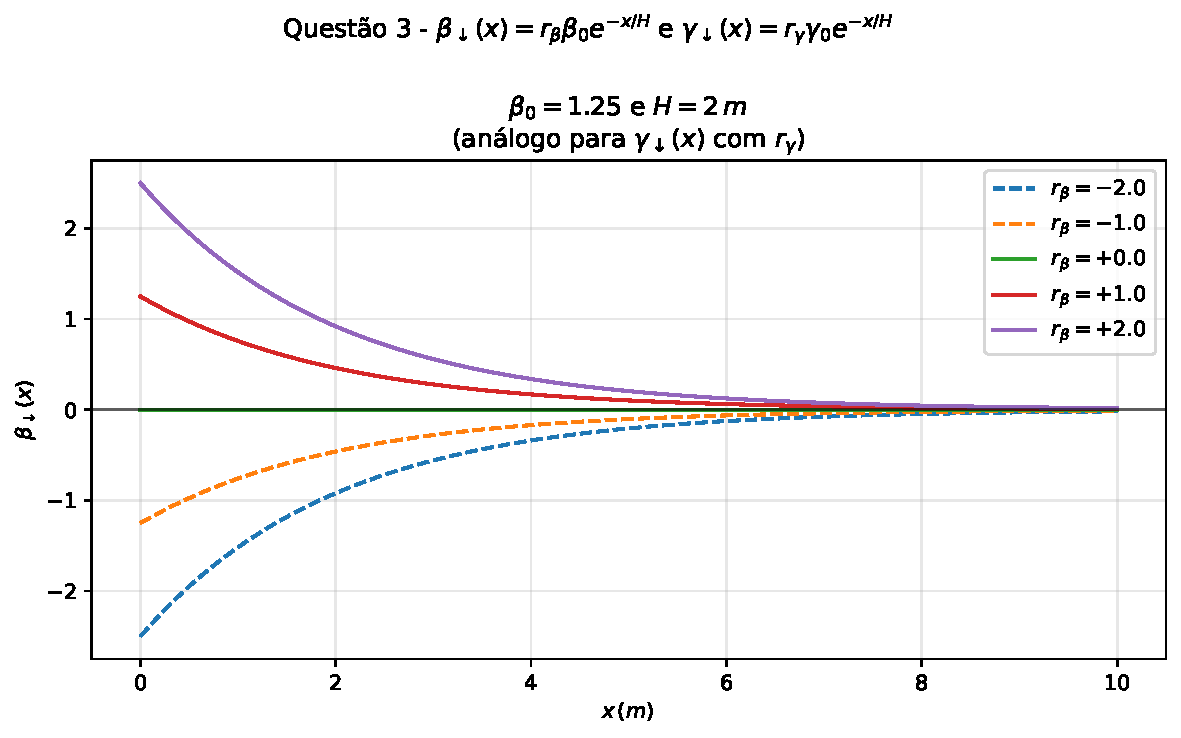
\includegraphics[width=0.75\linewidth]{Imagens/questao3_variacao_r_beta.pdf}
    \caption{Variação do $\beta_\downarrow$ pela altura}
    \label{fig:beta-down-variation}
\end{figure}

\subsection{Estrutura do Algoritmo de Integração Numérica}

\begin{questao}
Apresente um pseudocódigo contendo as estruturas principais para a integração numérica das equações
de movimento da partícula. Seu pseudocódigo deve incluir: inicialização das variáveis, definição dos
parâmetros, laço temporal e atualização de $x$ e $v$ a cada passo de tempo.
\end{questao}

A implementação organiza a simulação em duas partes, mostradas nos Algoritmos~\ref{alg:drag} e~\ref{alg:euler}. A força de arrasto (Alg.~\ref{alg:drag}) é encapsulada como uma função que recebe a partícula e devolve um vetor $\mathbb{R}^3$: o sinal de $v_z$ seleciona os coeficientes de subida ou descida, e a força resultante é sempre oposta ao vetor velocidade 3D. O laço principal (Alg.~\ref{alg:euler}) mantém uma lista de funções de força $\mathcal{F}$, soma suas contribuições a cada passo e aplica o método de Euler atualizando $\vec{v}$ \emph{antes} de $\vec{r}$ - caracterizando o Euler simplético. O estado é registrado antes de cada integração, e o laço termina quando $r_z < 0$.

\begin{algorithm}[H]
\caption{Força de arrasto - \texttt{drag\_force}}
\label{alg:drag}
\DontPrintSemicolon
\KwIn{Partícula $P$ $(\vec{r},\vec{v})$;\; parâmetros $\beta_0,\,\gamma_0,\,r_\beta,\,r_\gamma,\,H$}
\KwOut{Vetor força $\vec{F}_d \in \mathbb{R}^3$}
\BlankLine
$s \leftarrow \|\vec{v}\|$\tcp*{rapidez - norma 3D}
$\beta_\uparrow \leftarrow \beta_0\,e^{-r_z/H}$\;
$\gamma_\uparrow \leftarrow \gamma_0\,e^{-r_z/H}$\;
\BlankLine
\eIf{$v_z > 0$ \normalfont(subida)}{
    $\beta \leftarrow \beta_\uparrow$\;
    $\gamma \leftarrow \gamma_\uparrow$\;
}{
    $\beta \leftarrow r_\beta\,\beta_\uparrow$\;
    $\gamma \leftarrow r_\gamma\,\gamma_\uparrow$\;
}
\BlankLine
\KwRet{$\vec{v}\cdot(-\beta - \gamma\,s)$}\tcp*{força 3D, sempre oposta a $\vec{v}$}
\end{algorithm}

\begin{algorithm}[H]
\caption{Laço de integração - \texttt{simulate\_until\_ground}}
\label{alg:euler}
\DontPrintSemicolon
\KwIn{$m,\;\beta_0,\;\gamma_0,\;r_\beta,\;r_\gamma,\;H,\;\Delta t,\;\vec{r}_0,\;\vec{v}_0$}
\KwOut{Arrays $\vec{r}(t)$, $\vec{v}(t)$, $t$; métricas $x^*$, $\tau_\uparrow$, $\tau_\downarrow$, $\vec{v}^*$}
\BlankLine
inicializar $P$:\; $P.m \leftarrow m$;\; $P.\vec{r} \leftarrow \vec{r}_0$;\; $P.\vec{v} \leftarrow \vec{v}_0$\;
$\mathcal{F} \leftarrow \bigl[F_{\text{grav}}(a_g),\; F_{\text{drag}}(\beta_0,\gamma_0,r_\beta,r_\gamma,H)\bigr]$\tcp*{$F_\text{grav}$ usa $P.m$ internamente}
$t \leftarrow 0$\;
\BlankLine
\While{$P.r_z \geq 0$}{
    registrar $(t,\,P.\vec{r},\,P.\vec{v})$\tcp*{salva estado antes de integrar}
    \BlankLine
    $\vec{F} \leftarrow \displaystyle\sum_{f\,\in\,\mathcal{F}} f(P)$\tcp*{soma todas as forças}
    $P.\vec{v} \leftarrow P.\vec{v} + \dfrac{\vec{F}}{P.m}\,\Delta t$\tcp*{atualiza $\vec{v}$ primeiro}
    $P.\vec{r} \leftarrow P.\vec{r} + P.\vec{v}\,\Delta t$\tcp*{usa $\vec{v}$ já atualizado}
    $t \leftarrow t + \Delta t$\;
}
\BlankLine
\KwRet{arrays registrados + extrair métricas}
\end{algorithm}

\subsection{Implementação Numérica e Resultados}

\begin{questao}
Implemente o algoritmo em uma linguagem de programação de sua escolha e resolva numericamente
as equações de movimento para um conjunto de parâmetros fixos ($\beta_0$, $\gamma_0$, $r_\beta$, $r_\gamma$, $H$, etc.).
Apresente os resultados obtidos ($x(t)$ e $v(t)$) e discuta o comportamento da solução.

Nota: a integração numérica deve ser realizada em duas etapas distintas: uma correspondente à subida da partícula e outra à descida.
\end{questao}

O algoritmo foi implementado em Python utilizando integração de Euler simplético, com os parâmetros nominais da Tab.~\ref{tab:params-q6}. A Fig.~\ref{fig:simulation} compara as trajetórias obtidas com e sem arrasto em três painéis: a trajetória 3D no espaço, a posição vertical $z(t)$ e a velocidade vertical $v_z(t)$ ao longo do tempo.

\textbf{Trajetória 3D.} Sem arrasto, a partícula descreve uma parábola no espaço tridimensional; as componentes horizontais $x(t)$ e $y(t)$ crescem uniformemente (sem força horizontal), enquanto $z(t)$ segue um arco simétrico. Com arrasto, o movimento horizontal é também freado ao longo de todo o trajeto, resultando em um deslocamento horizontal menor e uma trajetória 3D mais compacta.

\textbf{Posição $z(t)$.} Sem arrasto, a curva é uma parábola simétrica: o tempo de subida é igual ao de descida e a altura máxima é maior. Com arrasto, a trajetória é assimétrica - a subida é mais curta (resistência soma-se à gravidade) e a descida é mais longa (arrasto assimétrico freia a queda). A altura máxima é reduzida.

\textbf{Velocidade vertical $v_z(t)$.} Sem arrasto, $v_z$ decresce linearmente até zero no ápice e cresce (em módulo) linearmente na queda, de forma completamente simétrica. Com arrasto, a desaceleração na subida é mais acentuada - ambas as forças atuam contra o movimento - enquanto na descida a aceleração é reduzida pela resistência assimétrica, resultando em uma velocidade de impacto $|v_z^*|$ muito inferior ao valor inicial $v_{z,0} = 12{,}0\,\text{m/s}$.

\begin{figure}[!htb]
    \centering
    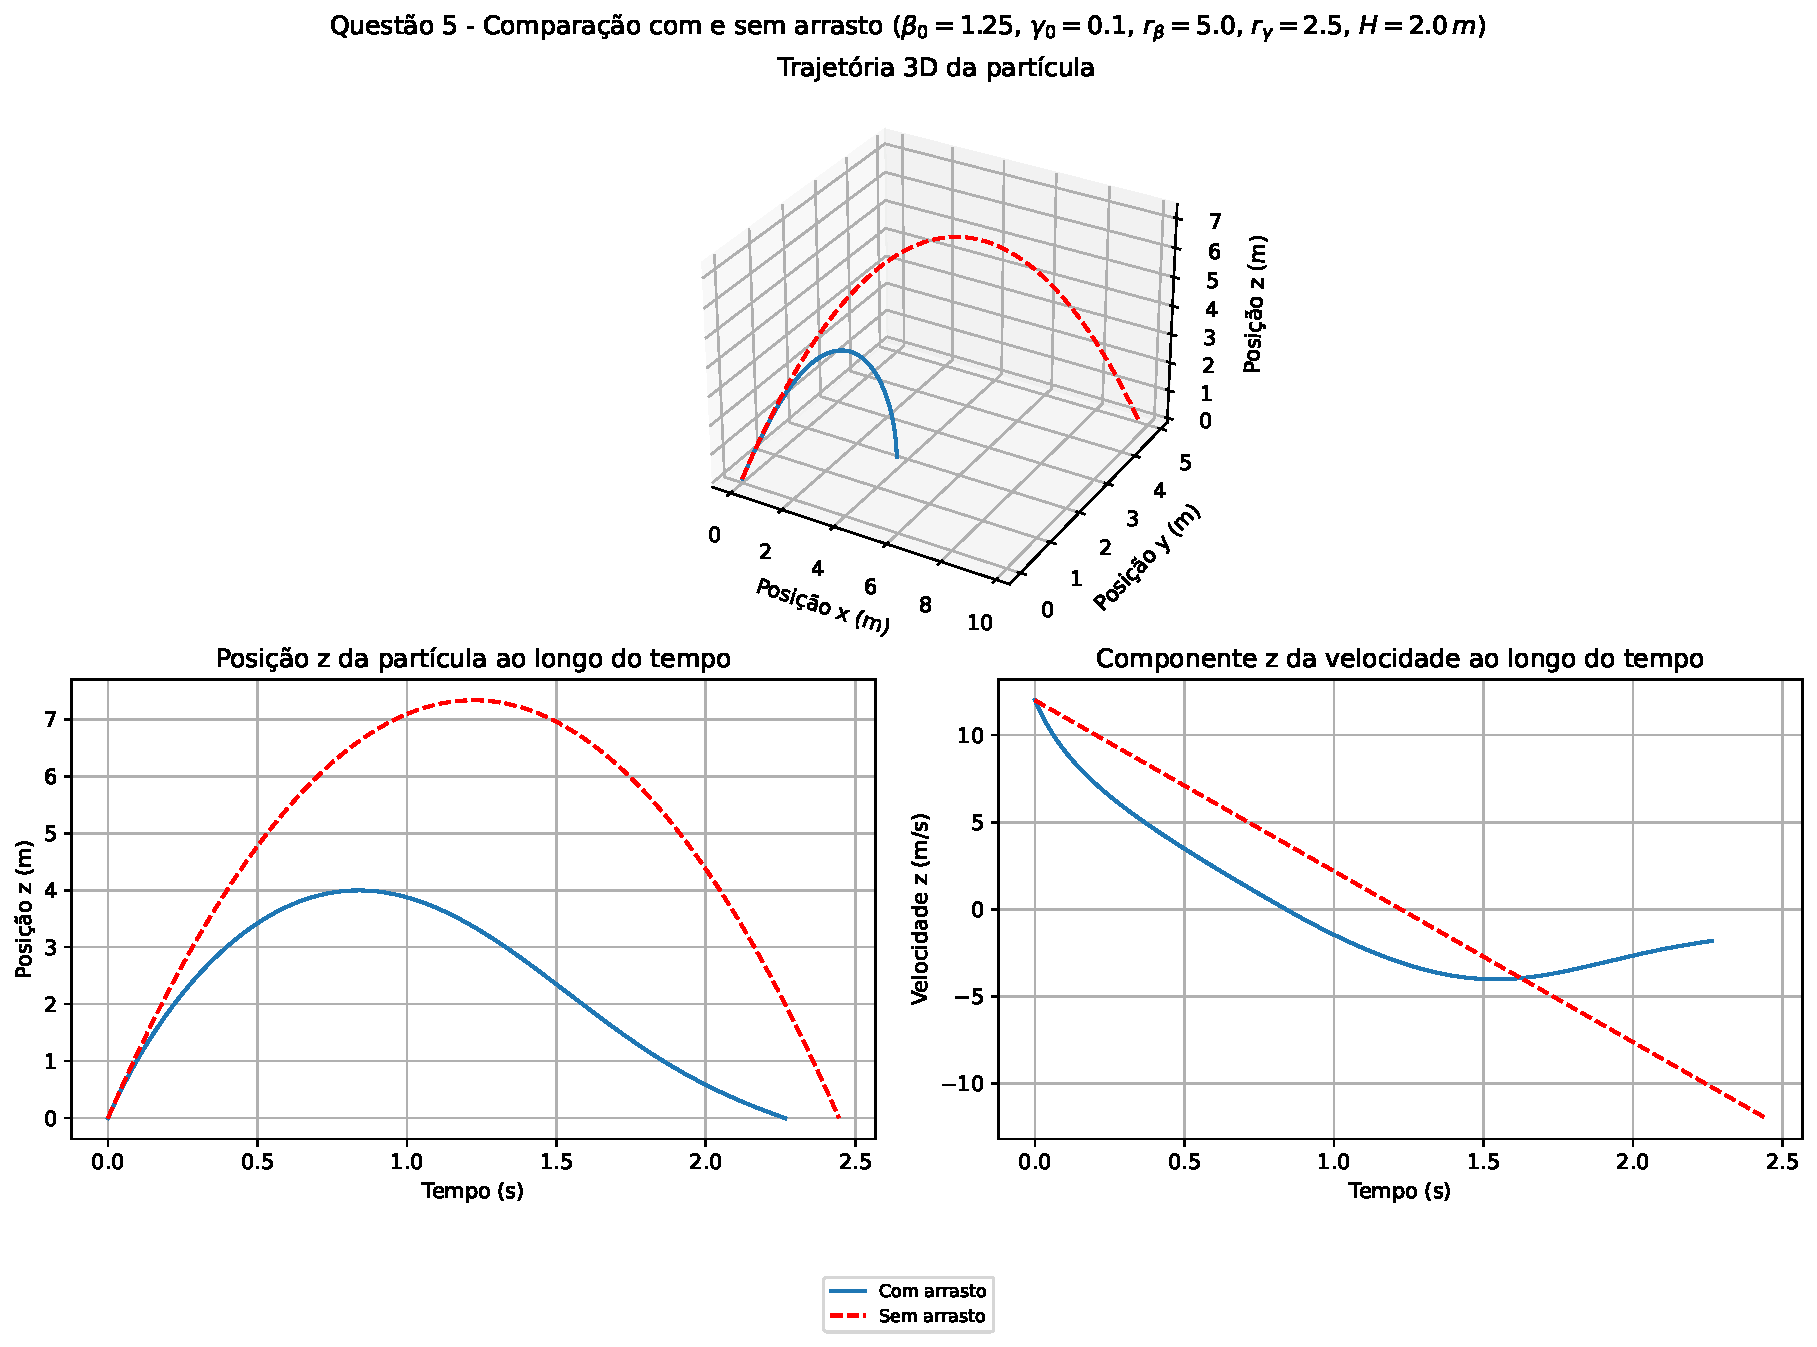
\includegraphics[width=\linewidth]{Imagens/comparacao_arrasto.pdf}
    \caption{Simulação da partícula, comparando trajetória com e sem arrasto}
    \label{fig:simulation}
\end{figure}


\subsection{Determinação de Grandezas Características}

\begin{questao}
A partir da solução numérica obtida, determine:

\begin{itemize}
    \item a altura máxima atingida pela partícula ($x^*$);
    \item a velocidade de impacto na descida ($v^*$) em $x = 0$;
    \item compare os tempos de subida ($\tau_\uparrow$) e descida ($\tau_\downarrow$).
\end{itemize}
\end{questao}

A simulação foi executada com os parâmetros listados na Tab.~\ref{tab:params-q6}, e os resultados obtidos são apresentados na Tab.~\ref{tab:results-q6}.

\begin{table}[!htb]
    \centering
    \caption{Parâmetros utilizados na simulação}
    \label{tab:params-q6}
    \begin{tabular}{llll}
        \hline
        Parâmetro & Símbolo & Valor & Unidade \\
        \hline
        Massa                         & $m$           & $1{,}0$  & kg \\
        Velocidade inicial            & $\vec{v}_0$   & $(4{,}0,\;2{,}0,\;12{,}0)$ & m/s \\
        Coef.\ arrasto linear         & $\beta_0$     & $1{,}25$ & kg/s \\
        Coef.\ arrasto quadrático     & $\gamma_0$    & $0{,}1$  & kg/m \\
        Assimetria linear             & $r_\beta$     & $5{,}0$  & - \\
        Assimetria quadrática         & $r_\gamma$    & $2{,}5$  & - \\
        Altura de escala              & $H$           & $2{,}0$  & m \\
        Passo de tempo                & $\Delta t$    & $0{,}001$& s \\
        \hline
    \end{tabular}
\end{table}

\begin{table}[!htb]
    \centering
    \caption{Grandezas características obtidas numericamente}
    \label{tab:results-q6}
    \begin{tabular}{lll}
        \hline
        Grandeza & Valor & Unidade \\
        \hline
        Altura máxima $x^*$                  & $3{,}996$ & m \\
        Tempo de subida $\tau_\uparrow$      & $0{,}838$ & s \\
        Tempo de descida $\tau_\downarrow$   & $1{,}427$ & s \\
        Velocidade de impacto $\vec{v}^*$    & $(0{,}033,\;0{,}016,\;-1{,}815)$ & m/s \\
        Módulo $|\vec{v}^*|$                 & $1{,}816$ & m/s \\
        \hline
    \end{tabular}
\end{table}

O tempo de descida ($\tau_\downarrow = 1{,}427\,\text{s}$) é significativamente maior que o de subida ($\tau_\uparrow = 0{,}838\,\text{s}$), numa razão de aproximadamente $1{,}70$. Esse resultado é esperado: durante a subida, arrasto e gravidade atuam no mesmo sentido (ambos opostos ao movimento), desacelerando a partícula rapidamente; durante a descida, a assimetria $r_\beta = 5{,}0$ intensifica o arrasto linear, reduzindo a aceleração líquida e prolongando o tempo de queda. A velocidade de impacto $|\vec{v}^*| = 1{,}816\,\text{m/s}$ é muito inferior ao módulo da velocidade inicial na componente vertical ($v_{z,0} = 12{,}0\,\text{m/s}$), confirmando que o arrasto dissipa grande parte da energia cinética ao longo da trajetória.


\subsection{Exploração Paramétrica do Sistema}

\begin{questao}
Realize uma exploração paramétrica do sistema. O objetivo é determinar a dependência de $x^*$,
$v^*$, $\tau_\uparrow$ e $\tau_\downarrow$ em função dos parâmetros $\beta_0$, $\gamma_0$, $r_\beta$, $r_\gamma$ e $H$. Escolha apenas um único parâmetro para variar, mantendo os demais fixos. Apresente os gráficos de
$x^*$, $v^*$, $\tau_\uparrow$ e $\tau_\downarrow$ em função do parâmetro escolhido. Exemplo: caso a escolha seja $r_\beta$, construa os gráficos de $x^*$, $v^*$, $\tau_\uparrow$
e $\tau_\downarrow$ em função de $r_\beta$. Discuta como variações nesses parâmetros influenciam as curvas obtidas.
\end{questao}

\begin{figure}[!htb]
    \centering
    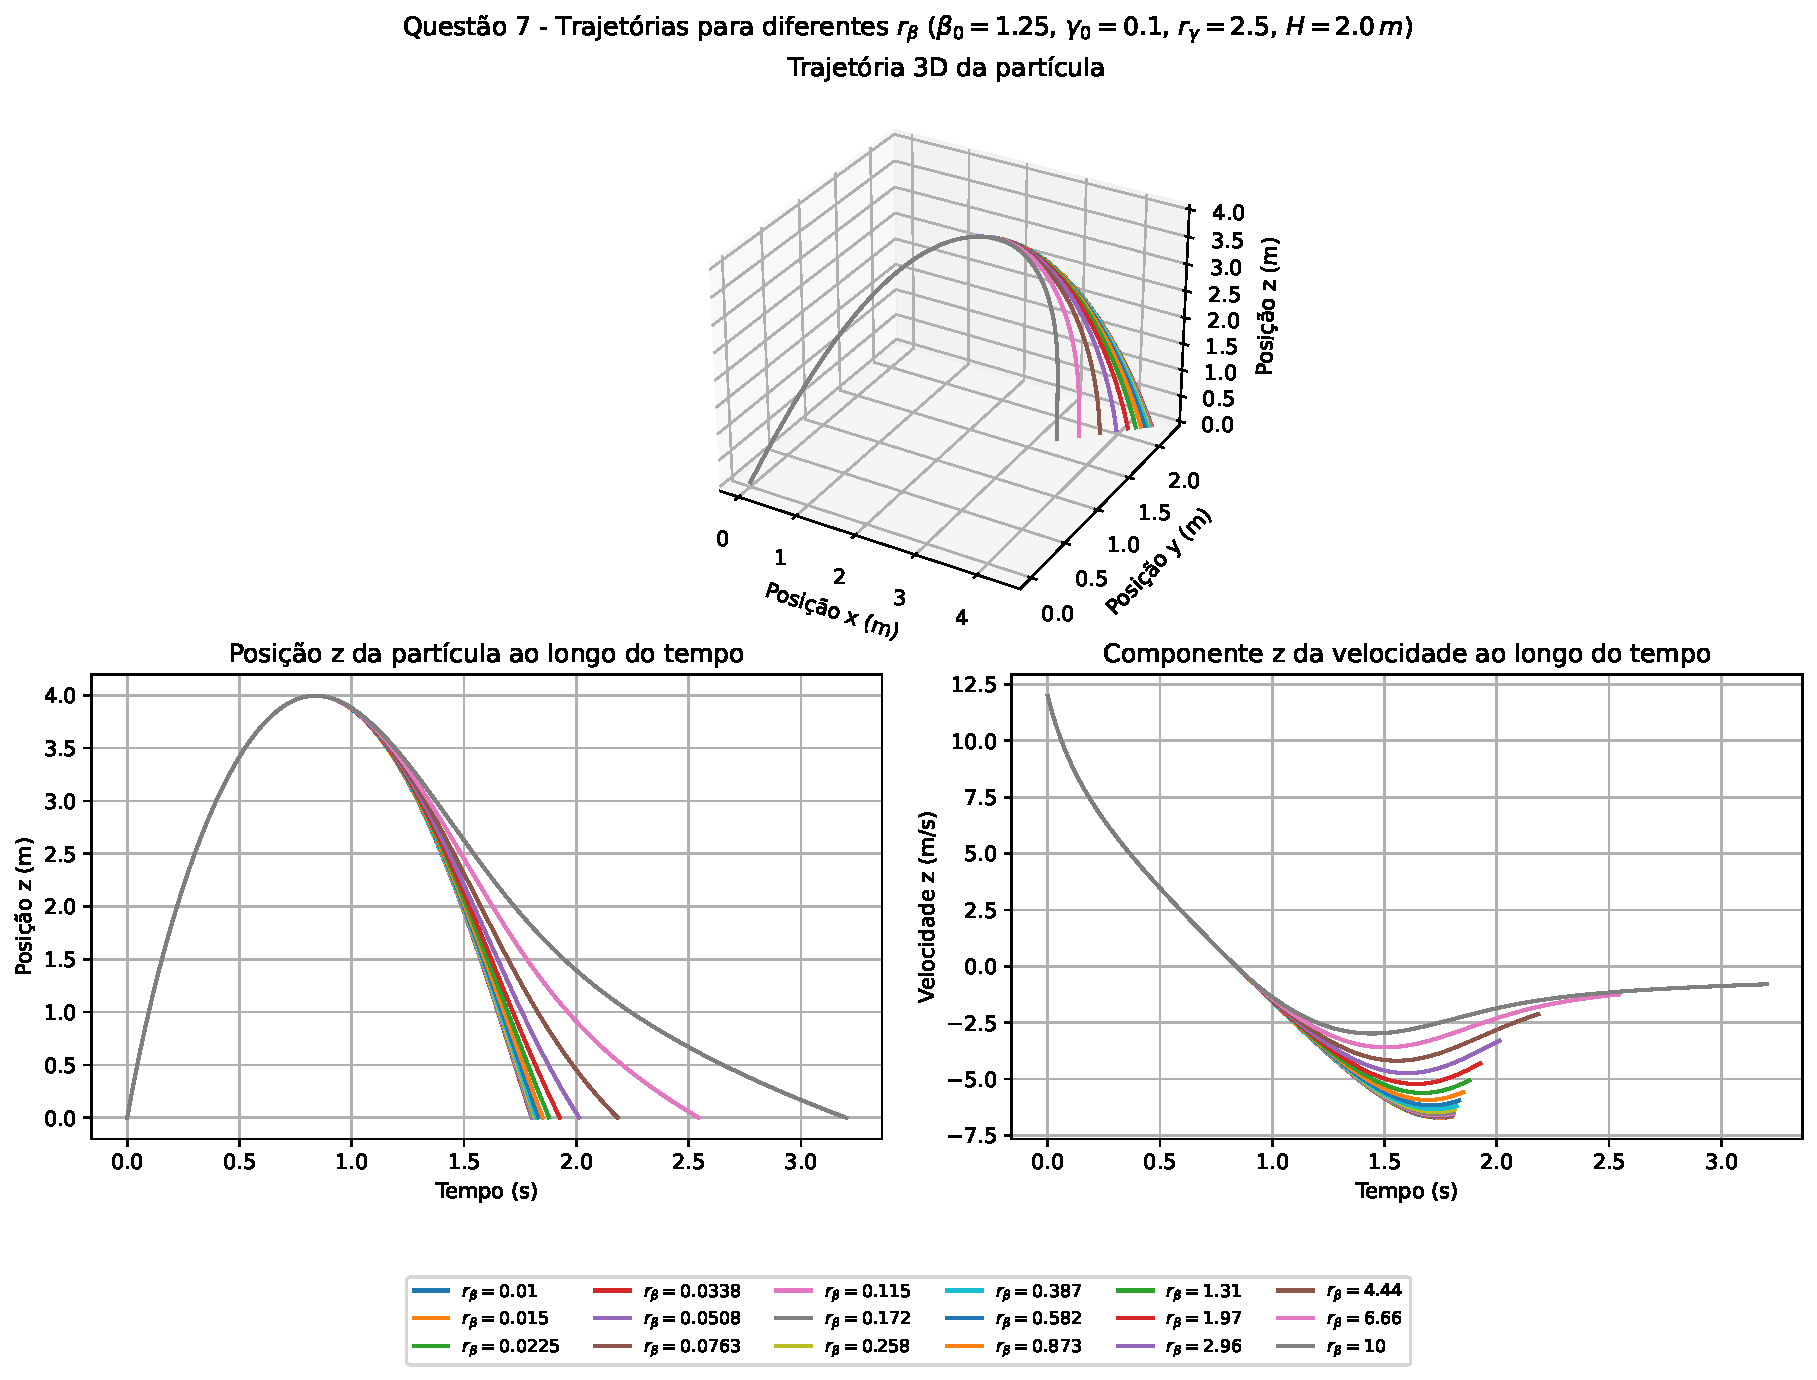
\includegraphics[width=\linewidth]{Imagens/questao7_r_beta_trajetorias.pdf}
    \caption{Trajetórias da partícula em função de $r_\beta$}
    \label{fig:particle-per-r_beta}
\end{figure}

O parâmetro escolhido para a exploração é $r_\beta$, variado no intervalo $r_\beta \in [0{,}01,\,10]$ em escala logarítmica com 18 pontos. Os demais parâmetros permanecem nos valores nominais: $\beta_0 = 1{,}25\,\text{kg/s}$, $\gamma_0 = 0{,}1\,\text{kg/m}$, $r_\gamma = 2{,}5$, $H = 2{,}0\,\text{m}$, com velocidade inicial $\vec{v}_0 = (4{,}0,\;2{,}0,\;12{,}0)\,\text{m/s}$ e massa $m = 1{,}0\,\text{kg}$.

\textbf{Trajetórias (Fig.~\ref{fig:particle-per-r_beta}).} Como $r_\beta$ entra exclusivamente nos coeficientes de descida - $\beta_\downarrow = r_\beta\,\beta_\uparrow$ e $\gamma_\downarrow = r_\gamma\,\gamma_\uparrow$ - e a condição de seleção é $v_z < 0$, a fase de \emph{subida} é completamente insensível a esse parâmetro. Consequentemente, todas as 18 trajetórias são sobrepostas durante a ascensão e começam a divergir apenas no momento em que a partícula inverte o sentido do movimento. Para $r_\beta$ pequeno ($r_\beta \approx 0{,}01$), o arrasto linear na descida é quase nulo; predomina apenas o arrasto quadrático via $r_\gamma$, e a partícula cai com maior aceleração, descrevendo uma trajetória descendente mais compacta. Para $r_\beta$ grande ($r_\beta \approx 10$), a componente linear $\beta_\downarrow$ passa a dominar, frenando progressivamente a partícula ao longo de toda a descida e produzindo trajetórias mais alongadas no eixo temporal.

\begin{figure}[!htb]
    \centering
    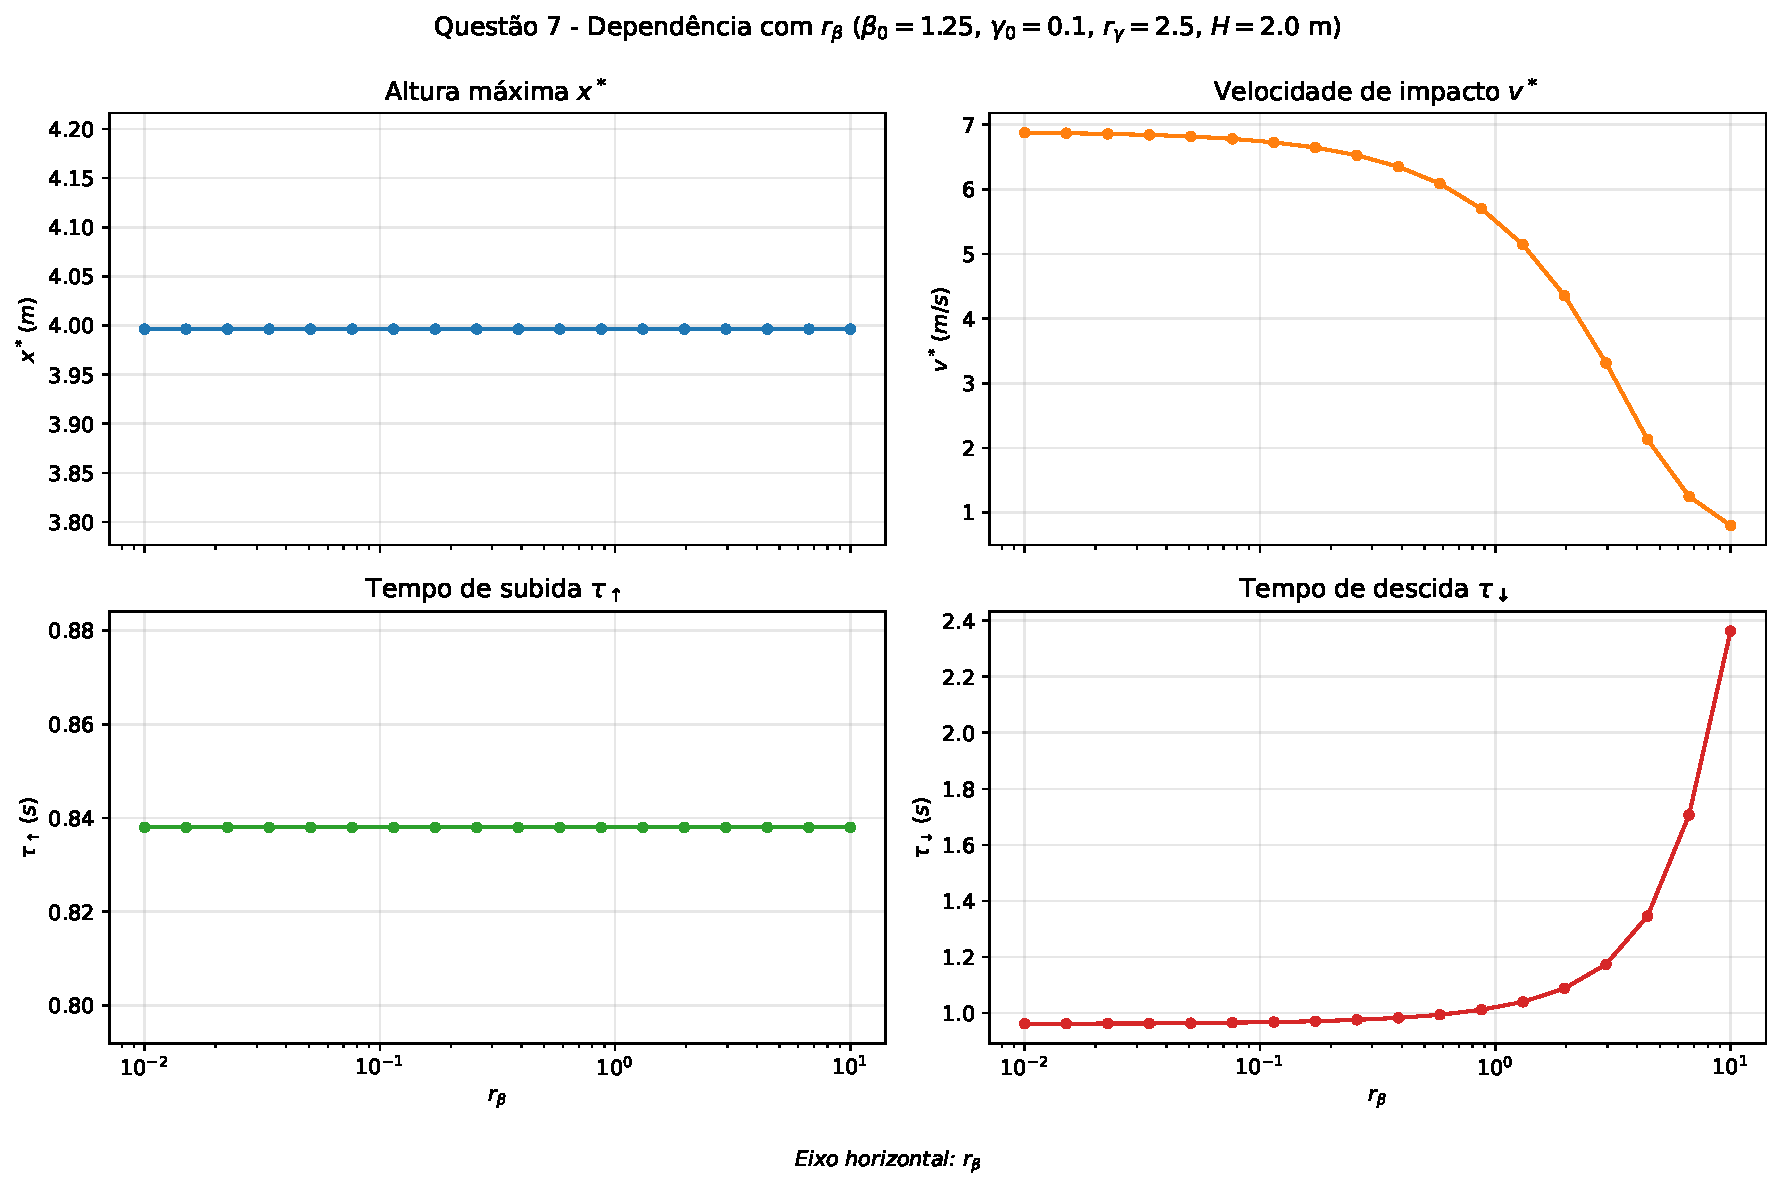
\includegraphics[width=\linewidth]{Imagens/questao7_r_beta_metricas.pdf}
    \caption{Métricas das trajetórias da partícula em função de $r_\beta$}
    \label{fig:metrics-particle-per-r_beta}
\end{figure}

\textbf{Métricas (Fig.~\ref{fig:metrics-particle-per-r_beta}).} A estrutura assimétrica do modelo se reflete diretamente nos quatro painéis:

\begin{itemize}
    \item \textbf{Altura máxima $x^*$}: linha plana para todo o intervalo de $r_\beta$. A altura máxima é determinada exclusivamente pela energia cinética inicial e pelo arrasto durante a subida; qualquer variação em $r_\beta$ é irrelevante para essa grandeza.

    \item \textbf{Tempo de subida $\tau_\uparrow$}: igualmente constante, pelo mesmo motivo. As curvas planas de $x^*$ e $\tau_\uparrow$ são uma consequência direta e verificável da separação entre as fases de subida e descida no modelo.

    \item \textbf{Velocidade de impacto $v^*$}: decresce monotonicamente com $r_\beta$. Para $r_\beta \to 0$, o amortecimento na descida é quase puramente quadrático ($r_\gamma = 2{,}5$) e $|v^*|$ se aproxima de seu valor máximo. À medida que $r_\beta$ cresce, o termo linear $\beta_\downarrow\,\|\vec{v}\|$ passa a dissipar mais energia ao longo da trajetória descendente, reduzindo progressivamente a velocidade de impacto. A curva apresenta uma variação suave em escala logarítmica, sugerindo que o efeito de $r_\beta$ é mais intenso na faixa $r_\beta \lesssim 1$ e satura gradualmente para valores maiores, à medida que a partícula se aproxima de uma velocidade terminal.

    \item \textbf{Tempo de descida $\tau_\downarrow$}: cresce monotonicamente com $r_\beta$, de forma complementar ao decrescimento de $v^*$. O aumento é mais acentuado para $r_\beta$ pequeno (onde o arrasto linear ainda é fraco) e mais suave para $r_\beta$ grande (onde a partícula já opera próxima da velocidade terminal durante parte da queda).
\end{itemize}


Para o valor nominal $r_\beta = 5{,}0$, os resultados da Tab.~\ref{tab:results-q6} mostram $\tau_\downarrow/\tau_\uparrow \approx 1{,}70$: a descida é 70\% mais lenta que a subida, refletindo a intensidade do arrasto assimétrico escolhido. A exploração paramétrica demonstra que essa razão pode ser ajustada continuamente através de $r_\beta$, o que torna esse parâmetro o principal mecanismo de controle da assimetria temporal da trajetória no modelo.
